\documentclass[conference]{IEEEtran}
\IEEEoverridecommandlockouts
% The preceding line is only needed to identify funding in the first footnote. If that is unneeded, please comment it out.
\usepackage{ctex}
\usepackage{algorithm}
\usepackage[noend]{algpseudocode}
\usepackage{cite}
\usepackage{amsmath,amssymb,amsfonts}
\usepackage{graphicx}
\usepackage{textcomp}
\usepackage{xcolor}
\def\BibTeX{{\rm B\kern-.05em{\sc i\kern-.025em b}\kern-.08em
    T\kern-.1667em\lower.7ex\hbox{E}\kern-.125emX}}
\begin{document}

\title{Resource Management in Large Language Models\\
    \thanks{Identify applicable funding agency here. If none, delete this.}
}

\author{\IEEEauthorblockN{{\kaishu 朱徐洲}}
    \IEEEauthorblockA{522031910324}
    \IEEEauthorblockA{zhuxuzhou@sjtu.edu.cn}
    \and
    \IEEEauthorblockN{{\kaishu 庞皓阳}}
    \IEEEauthorblockA{522031910050}
    \IEEEauthorblockA{1271362703@sjtu.edu.cn}
    \and
    \IEEEauthorblockN{{\kaishu 卢晗宇}}
    \IEEEauthorblockA{522031910043}
    \IEEEauthorblockA{lhy-2785.fanyang@sjtu.edu.cn}
}

\maketitle

\begin{abstract}
    In recent years, there has been a continuous evolution in the scale, performance, and applications of large language models (LLMs),\\
    progressing from initial models with several million parameters to current models with tens to hundreds of billions of parameters. \\
    These advancements have led to a continual enhancement in their language understanding and generation capabilities, facilitating their \\
    widespread adoption across domains such as natural language processing, intelligent customer service, and automated writing. \\
    Concurrently, trends in transfer learning and open-source sharing have further propelled their applicability and adaptability \\
    across specific tasks and domains. However, as the parameter count escalates, the demand for computational and storage resources also increases, \\
    posing a series of challenges and bottlenecks. This survey aims to analyze the existing issues and relevant research efforts in memory management, process scheduling, and computational resource allocation, offering comprehensive insights and valuable perspectives derived from existing literature.
\end{abstract}

\begin{IEEEkeywords}
    LLM, Transformer, Memory Management, Attention Mechanism, Process Scheduling, Distributed Training, Offloading, Inference
\end{IEEEkeywords}

\section{Introduction}
During the operation of LLMs, the memory requirements are complex and substantial. In the model training phase, memory is needed for model parameters and gradients, activation values, and optimizer states. During the inference phase, memory is required for model parameters and input data buffers. Recently, as the demand for long-sequence inference has grown, the proportion of memory occupied by the Key-Value cache has increased in order to maintain more contextual information, becoming a focal point for memory optimization.
Therefore, efficient memory allocation is crucial for large language models. Memory not only affects data storage but also plays a crucial role in improving the training and inference speed of the model, reducing memory footprint and resource allocation, and preventing memory leaks.

The Transformer model has achieved tremendous success in the field of Natural Language Processing (NLP) and has become the foundational architecture for many powerful pre-trained language models, such as BERT and GPT. LLMs typically rely on the Transformer architecture and leverage massive corpora for pre-training to learn rich representations of language. Thus, LLMs can be viewed as specific applications of the Transformer model in NLP tasks. However, advanced models may have large volumes and require significant resources, resulting in high usage costs. For instance, GPT-3 has 175 billion parameters, and serving models of such scale may incur substantial costs due to computational expenses, necessitating acceleration from the perspective of process management and scheduling.
The inference of LLMs is constrained by memory input/output (I/O) limitations rather than computational constraints. In other words, currently, the time required to load 1MB of data into the computing cores of a GPU is greater than the time these computing cores need to perform LLM computations on 1MB of data. This implies that the throughput of LLM inference is largely dependent on how much batch processing can be accommodated within the high-bandwidth GPU memory.
\section{memory management}
\subsection{Memory Optimization Based on the Attention Algorithm}
This section primarily focuses on the Attention algorithm, which essentially involves optimizing memory management for the Key-Value (KV) cache.
\subsubsection{PagedAttention}
In long-sequence inference, the KV cache accumulates a significant amount of contextual information regarding keys and values, resulting in substantial memory consumption that dynamically fluctuates, akin to memory allocation challenges encountered in operating systems. Classic OS memory management techniques, like virtual memory and paging, effectively mitigate unnecessary memory usage, enhancing memory utilization. These principles can inform the design of LLMs.

Within the Transformer architecture and its derivatives, the attention mechanism serves as a crucial component for enabling the model to comprehend the relationships among input data. Consequently, integrating paging concepts, like paging the KV cache, should be contemplated within the Attention algorithm. The PagedAttention algorithm[1], proposed by Woosuk Kwon and colleagues, offers an illustrative implementation method. Leveraging this insight, vLLM, a service system tailored for LLMs, has been developed.

vLLM is based on the PagedAttention algorithm. The strategy of PagedAttention involves dividing the KV cache of each sequence into multiple blocks, each containing a certain number of tokens' keys and values. For each request to the KV cache, multiple non-contiguous blocks can be allocated. Figure 1 illustrates the storage method of keys and values in the KV cache under the PagedAttention algorithm, while also demonstrating the computation of Query and Key under this storage format.

\begin{figure}[htbp]
    \centerline{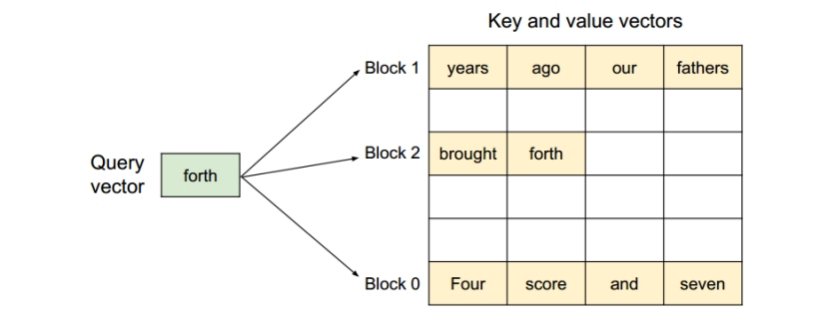
\includegraphics[width=0.5\textwidth]{process figM1.png}}
    \caption{The block storage in the PagedAttention [2]}
    \label{fig}
\end{figure}

After dividing the KV cache, the original k and v values in the self-attention calculation formula are transformed into k and v vectors corresponding to the blocks in which they are stored. The formula is modified as follows:

\[a_{ij} = \frac{\exp(q_i^{T} \cdot k_j / \sqrt{d})}{\sum_{t=1}^{i} \exp(q_i^{T} \cdot k_t / \sqrt{d})}, \quad o_i = \sum_{j=1}^{i} a_{ij} v_j\]

\[A_{ij} = \frac{\exp(q_i^{T} \cdot K_j / \sqrt{d})}{\sum_{t=1}^{\lceil {i/B} \rceil} \exp(q_i^{T} \cdot K_t1 / \sqrt{d})}, \quad o_i = \sum_{j=1}^{\lceil {i/B} \rceil} V_j A_{ij}^{T}\]

vLLM employs block-level memory management and preemptive request scheduling, both of which are co-designed with PagedAttention. A request’s KV cache is represented as a series of logical KV blocks, filled from left to right as new tokens and their KV cache are generated. Just like the page table in operating system, the KV block manager maintains block tables. Each block table entry records the corresponding physical blocks of a logical block and the number of filled positions. Moreover, the vLLM’s block table has a “filled” record for each block, which represents the number of tokens in that block. If the “filled” record does not equal the maximum capacity that each block can accommodate, then when the key and value of a new token need to be added to the KV cache, the system will first attempt to fill any vacancies in the previous block.

The concept of partitioning the KV cache allows for similar benefits in optimizing KV cache storage space: the space can be non-contiguous, eliminating the external fragmentation caused by contiguous storage. Additionally, the “filled” records also maximize the utilization of each block to a certain extent, thereby reducing internal fragmentation. Moreover, the PagedAttention kernel can process the KV cache in parallel across multiple positions, thereby enhancing hardware utilization and reducing latency.

\subsubsection{Self-Analysis: Combination of vLLM and distributed storage}
In vLLM, using a centralized scheduler to coordinate parallel model execution is crucial. This strategy ensures that each model shard can efficiently handle the tasks assigned to it. In this setup, although each GPU processes a part of the entire input, all GPUs still need to access the same set of KV cache data. Therefore, vLLM adopts a centrally managed single KV cache manager to synchronize and share critical data across all computing nodes.

vLLM's design is highly suitable for integration with distributed storage systems, offering the some key advantages: vLLM can implement block allocation and dynamic management of the KV cache. When integrated with distributed storage systems, this architecture can leverage the storage system's dynamic resource allocation capabilities, automatically expanding or contracting storage resources as needed. This not only improves memory utilization but also increases the system's total storage capacity. It also helps to store data close to the computing resources that use this data, thereby reducing data transmission times and enhancing overall processing speed. Moreover, this combination can utilize advanced data backup and fault tolerance mechanisms. In the event of a single node or device failure, the system can automatically recover KV cache data from backups.


\subsubsection{Tree Attention}
In traditional LLMs, keys and values for each output sequence are independently calculated and stored in a kv cache, lacking effective data sharing among sequences with the same prefixes. We can envision tokens as nodes in a tree, facilitating sharing and reuse of computed k and v values during generation.

An example of this idea's application is the SpecInfer engine[3], which employs a "Small Speculative Model" (SSM) for tentative speculative inference, depicted in Figure 2. Efficient tree decoding operators enable parallelized inference, and verified paths are output as the model's inference result sequence.

\begin{figure}[htbp]
    \centerline{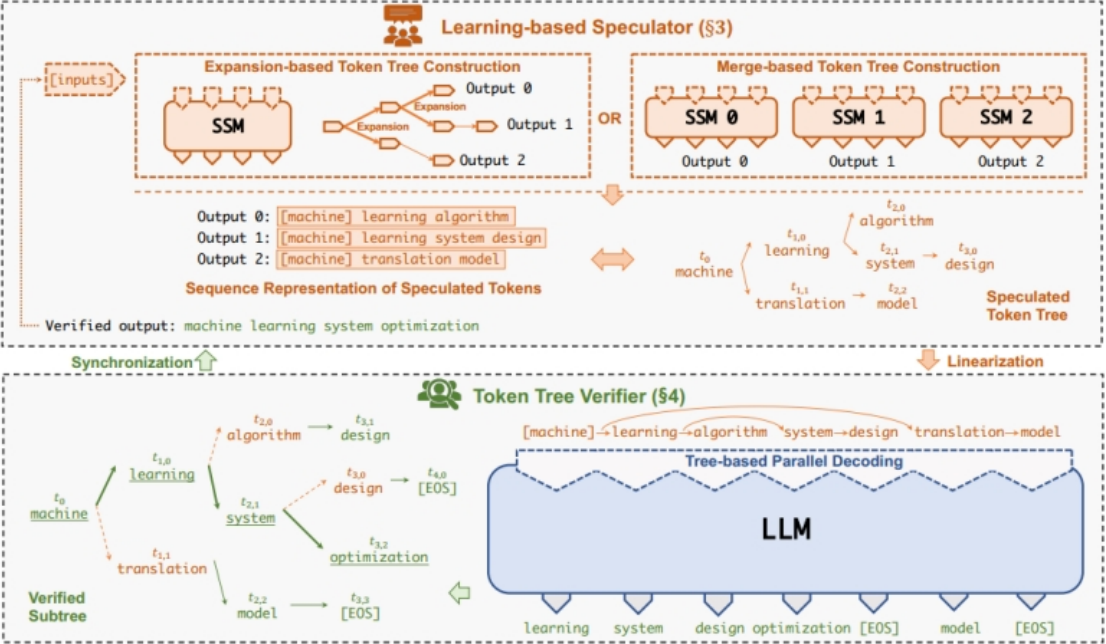
\includegraphics[width=0.5\textwidth]{process figM2.png}}
    \caption{An overview of SpecInfer's tree based speculative inference and verification mechanism [4]}
    \label{fig}
\end{figure}

Before Tree Attention, SpecInfer breaks down sentences into tokens and utilizes SSM to construct candidate token sequences layer by layer from the root node.

During Tree Attention validation, each candidate token sequence's accuracy must be verified. It calculates probability scores for sequences by appending possible subsequent tokens to the current prefix, achieving parallel verification of multiple tokens. This method allows reuse of k and v values in each layer's computation, reducing memory consumption by avoiding duplicate storage.

Integrating Tree Attention with DFS effectively eliminates redundant KV cache allocations from multiple output sequences sharing the same prefixes, significantly enhancing memory utilization and computational efficiency.

\subsubsection{Summary of Attention Algorithm}
When employing memory optimization strategies based on attention mechanisms, the reduction in memory usage is often not significant, but there is usually a substantial increase in the inference time for LLMs. Essentially, this strategy involves trading time for space. Therefore, when implementing such optimizations, it is crucial to balance computational performance and memory efficiency, making decisions based on specific application requirements.

\subsection{Memory Management in Long-Term Memory and Recall}
In the description above, the term "memory" has two different meanings. The first "memory" refers to the computer's hardware resources, while the second "memory" refers to the recollection of key contextual information that LLMs need to retain when processing lengthy texts.
\subsubsection{Background}
With the development of LLMs, the datasets they rely on have become increasingly vast, and the input they process has become more verbose. When faced with massive amounts of input data, the model's original context-linking capabilities might experience a "forgetting" phenomenon, which is the loss of crucial historical information. To address this issue, memory modules were developed. These modules have become effective tools for handling long-term dependencies, enhancing understanding of context, and improving memory of past information.

There are several main types of memory modules in LLMs. The following will provide a detailed analysis of a specific memory module design called “Self-Controlled Memory System”(SCM)[5].

\subsubsection{Implementation and Benefits of SCM}
The SCM system optimizes LLM processing and responsiveness, particularly in memory management. It efficiently stores structured memory items like interaction indices, observations, responses, summaries, and embeddings using caching and vector databases. Memories are categorized into Activation Memory for historical data and Flash Memory for recent interactions, allowing flexible memory utilization.

Memory Activation in the Memory Controller relies on prompts to activate historical memories based on the model's response to current observations. Memories are retrieved and ranked by recency and relevance scores computed from cosine similarity between query and memory embeddings. Only the top k memories (3 to 10) are activated, ensuring pertinent and recent memories are utilized.

Summaries are employed to represent memories if activated memory tokens exceed 2000 and memory length exceeds 800 tokens, reducing data processing volume and maintaining the model within its maximum input length capacity.

\subsubsection{Personal Extended Ideas}
Given the extensive range of memory module designs in LLMs, I have not yet fully explored all these designs. Based on my current knowledge and preliminary understanding of this field, here are some of my thoughts and ideas on memory optimization.

Eviction Policies:

Implementing eviction mechanisms to remove memories that have not been used for an extended period can effectively reduce space consumption. This strategy is analogous to cache eviction algorithms in computer systems and allows for dynamic memory management, ensuring operational efficiency.

Memory Pooling:

Manage memory allocations using memory pools to reduce the overhead associated with frequent memory allocation and deallocation. Memory pools pre-allocate a large block of memory and dynamically allocate or reclaim memory from this block as needed.

Garbage Collection Optimization:

Optimize garbage collection (GC) mechanisms to minimize their impact on system performance. By improving GC algorithms, memory can be managed more effectively without sacrificing response times.

Heterogeneous Storage Strategies:

Employ a combination of different types of storage media (e.g., RAM, SSD, HDD) to store data with varying access frequencies. Frequently accessed "hot" data can be stored on faster media like RAM, while "cold" data can be placed on lower-cost media like HDD.



\section{process scheduling}

Inference serving plays a pivotal role in the functionality of interactive AI applications based on LLMs, demanding low job completion times (JCT) to ensure an engaging user experience. However, the substantial size and complexity of LLMs present challenges to inference serving infrastructure, often requiring enterprises to deploy costly clusters equipped with accelerators like GPUs and TPUs. LLM inference possesses unique characteristics that set it apart from other deep neural network (DNN) model inference tasks, such as ResNet【6】. While DNN inference jobs are typically deterministic and highly predictable 【7】, LLM inference follows a distinct autoregressive pattern. Each iteration of an LLM inference job generates one output token, which is then appended to the input for producing the next output token in the subsequent iteration. The execution time of LLM inference depends on both the input and output lengths, with the latter being unknown beforehand, and that also gives a direction of optimizing.
Therefore, we start from the Transformer model and analyze various process management and scheduling methods available.


\subsection{iteration-level scheduling in Orca}
\subsubsection{problems to be solved}


Due to the large scale of models and texts, batch processing is employed to improve efficiency. Traditional LLM serving systems adopt a run-to-completion approach, where a task continues execution until completion without interruption or pause. However, this approach presents issues:
- The input lengths vary, and different requests may require different numbers of iterations, causing some requests to complete prematurely.
Assume there are two requests named x1 and x2. x1 carries a string of “I think this is great”. x2 carries a string of “I love you”. We send the two requests to the transformer
\begin{figure}[htbp]
    \centerline{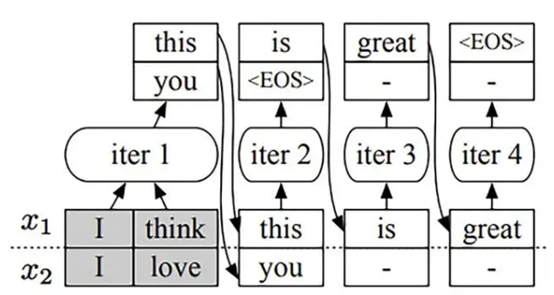
\includegraphics[width=0.5\textwidth]{process fig1.png}}
    \caption{scheduling execution at the request granularity level}
    \label{fig}
\end{figure}
The figure illustrates the scheduling execution at the request granularity level. In this scenario,
although request x2 finishes earlier than request x1, the engine performs computation for both “active” and “inactive” requests throughout all iterations. Such extra computation for inactive requests (x2 at iter 3 and 4) limits the efficiency of batched execution. What makes it even worse is that this behavior prevents an early return of the finished request to the client, imposing a substantial amount of extra latency. This is because the engine only returns the execution results to the serving system when it finishes processing all requests in the batch. Similarly, when a new request arrives in the middle of the current batch’s execution, the newly arrived request must wait until all requests in the current batch have finished. Therefore, this will incur a significant amount of additional computational costs and time overhead. [1]


\subsubsection{Solution: iteration-level scheduling}


Orca gives a distributed serving system which is utilized for deploying Transformer-based generative models.


Orca addresses this by scheduling each request at a finer granularity (i.e., at each iteration), in FCFS order:
- The iteration-level scheduler repeats the following three steps:
- Selects requests to run next.
- Invokes the engine to execute one iteration for the selected requests.
- Receives execution results for the scheduled iteration.

When the scheduler receives returns after each iteration, it can detect the completion status of requests, promptly returning completed requests to the client. Importantly, new incoming requests only need to wait for one iteration, significantly reducing queuing delays.

\subsubsection{Benefits transferability of the iteration-level scheduling strategy}


The transition of the serving system from request granularity to implementing scheduling at each iteration granularity has enhanced overall scheduling flexibility and improved utilization of computational resources.
The scheduler monitors the completion status of requests at each iteration, allowing each completed request to return immediately without waiting for other requests to finish together. The space freed up by returned requests enables new incoming requests to enter, significantly reducing queuing delays.

According to evaluation on a GPT-3 175B model , Orca can significantly outperform NVIDIA FasterTransformer in terms of both latency and throughput: 36.9X throughput improvement at the same level of latency.[1]


The ability of Large Language Models (LLMs) to perform iteration-level process scheduling and its transferability across different LLM architectures stem from their intrinsic model-agnostic nature. Such scheduling methodologies operate independently of the internal structure of the models, focusing instead on task partitioning and management during iterative computations. Leveraging the parallelism inherent in LLM iterative computations, these scheduling approaches efficiently distribute tasks, irrespective of model specifics, thereby facilitating their migration across diverse LLM frameworks. Furthermore, the reliance on task similarities and the adaptability of scheduling algorithms enable seamless transition and optimization across model boundaries, ensuring their applicability in varied academic contexts.

Thus the iteration-level batch processing (also known as continuous batch processing) method is versatile and can be applied to other models as well, and three examples are shown here:
- Utilizing continuous batch processing and model-specific memory optimizations (using vLLM) can increase throughput by up to 23 times. [2]
- Throughput with continuous batch processing (in Ray Serve and Hugging Face's text generation inference) is 8 times that of naive batch processing. [3]
- By employing optimized models (such as NVIDIA's FasterTransformer), throughput can be increased by 4 times compared to naive batch processing. [3]

\subsection{FastServe}
\subsubsection{problems to be solved}

Orca implementations used an FCFS strategy without preemptive mechanisms, meaning once a job enters the running state, it must wait until completion. This leads to severe head-of-line blocking issues,which indicates a phenomenon that the delivery of certain packets or tasks is delayed due to the presence of other packets or tasks ahead of them in the queue. Therefore, FastServe, a distributed inference serving system for LLMs, adopts a skip-join Multi-Level Feedback Queue scheduler to implement preemptive scheduling.
\subsubsection{Skip-join Multi-Level Feedback Queue scheduler}


FastServe is based on a preemptive Multi-Level Feedback Queue, where each job initially enters the highest-level queue and gradually descends to lower priority queues as it consumes its time slice, reducing job completion time. To avoid starving, a promote mechanism periodically promotes some jobs. Specifically, each job sets a starve timer, and if it waits in the waiting state beyond a threshold, it is promoted to the highest-level queue Q1. Finally, the scheduler selects jobs for execution based on queue priority from highest to lowest.

\begin{algorithm}
    \caption{Skip-Join MLFQ Scheduler}
    \begin{algorithmic}[1]
        \State \textbf{Input:} Queues $Q_1, Q_2, ..., Q_k$, jobs $J_{in}$, $J_{pre}$, profiling info $P$
        \State \textbf{Output:} Jobs to be executed $J_{out}$
        \Procedure{SkipJoinMLFQScheduler}{}
        \State \textbf{Initialization:} $J_{out} \leftarrow \emptyset$
        \For{$job \in J_{in}$}
        \State $nextIterTime \leftarrow P.getNextIterationTime(job)$, $p_{job} \leftarrow getHighestPriority(nextIterTime)$
        \State $Q_{p_{job}}.push(job)$
        \EndFor
        \For{$job \in J_{pre}$}
        \State $job.outputNextGeneratedToken()$, $p_{job} \leftarrow job.getCurrentPriority()$
        \If{$job.isFinished()$}
        \State $Q_{p_{job}}.pop(job)$
        \State \textbf{continue}
        \EndIf
        \If{$job.needsDemotion()$}
        \State $nextIterTime' \leftarrow P.getNextIterationTime(job)$
        \State $p_{job} \leftarrow getDemotionPriority(p_{job}, nextIterTime')$, $r.demoteTo(Q_{p_{job}})$
        \EndIf
        \EndFor
        \For{$q \in \{Q_2, Q_3, ..., Q_k\}$}
        \For{$job \in q$}
        \If{$job.needsPromotion()$}
        \State $job.promoteTo(Q_1)$, $job.reserveTime()$
        \EndIf
        \EndFor
        \EndFor
        \For{$q \in \{Q_1, Q_2, ..., Q_k\}$}
        \For{$job \in q$}
        \If{$job.isReady()$ and $|J_{out}| < MaxBatchSize$}
        \State $J_{out}.push(job)$
        \EndIf
        \EndFor
        \EndFor
        \EndProcedure
    \end{algorithmic}
\end{algorithm}
In MLFQ eviction, a skip-join mechanism is introduced. Before a new job joins the queue, it is evaluated (the reason is explained in next paragraph), and based on the estimated overall execution time using prefill time, it is placed into different priority queues. This aims to prioritize the execution of projects with the least remaining time.

\begin{figure}[htbp]
    \centerline{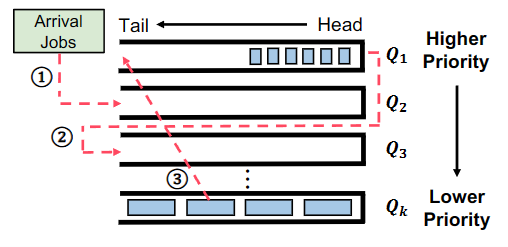
\includegraphics[width=0.5\textwidth]{process fig4.png}}
    \caption{Skip-join MLFQ with starvation prevention}
    \label{fig}
\end{figure}

Specifically, although the number of iterations (i.e., the output length) is not known ahead of time, the execution time of each iteration is predictable. The iteration time is determined by a few key parameters suchas the hardware, the model, and the input length, and thus
can be accurately profiled in advance. Figure below shows the iteration time for GPT-3 2.7B on NVIDIA A100 under different input sequence length. We can see that the first iteration
time (i.e., the execution time to generate the first output token) is longer than those in the decoding phase within a single job. As the input sequence length increases, the first iteration time grows roughly in a linear manner, while the increase of the iteration time in the decoding phase is negligible. This gives the skip-join mechanism information, so the algorithm can decide which queue the new job joins.

\begin{figure}[htbp]
    \centerline{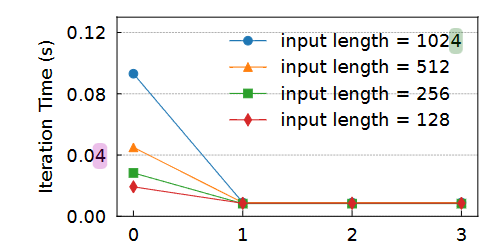
\includegraphics[width=0.5\textwidth]{process fig5.png}}
    \caption{ The execution time of the first four iterations (i.e.first four output tokens) with different input sequence length}
    \label{fig}
\end{figure}

\subsection*{Benefits and drawbacks of the strategy}

\section*{Acknowledgment}


The preferred spelling of the word ``acknowledgment'' in America is without
an ``e'' after the ``g''. Avoid the stilted expression ``one of us (R. B.
G.) thanks $\ldots$''. Instead, try ``R. B. G. thanks$\ldots$''. Put sponsor
acknowledgments in the unnumbered footnote on the first page.

\section*{References}

Please number citations consecutively within brackets \cite{b1}. The
sentence punctuation follows the bracket \cite{b2}. Refer simply to the reference
number, as in \cite{b3}---do not use ``Ref. \cite{b3}'' or ``reference \cite{b3}'' except at
the beginning of a sentence: ``Reference \cite{b3} was the first $\ldots$''

Number footnotes separately in superscripts. Place the actual footnote at
the bottom of the column in which it was cited. Do not put footnotes in the
abstract or reference list. Use letters for table footnotes.

Unless there are six authors or more give all authors' names; do not use
``et al.''. Papers that have not been published, even if they have been
submitted for publication, should be cited as ``unpublished'' \cite{b4}. Papers
that have been accepted for publication should be cited as ``in press'' \cite{b5}.
Capitalize only the first word in a paper title, except for proper nouns and
element symbols.

For papers published in translation journals, please give the English
citation first, followed by the original foreign-language citation \cite{b6}.

\begin{thebibliography}{00}
    \bibitem{b1} Kwon W, Li Z, Zhuang S, et al. Efficient memory management for large language model serving with pagedattention[C]//Proceedings of the 29th Symposium on Operating Systems Principles. 2023: 611-626.
    \bibitem{b2} Kwon W, Li Z, Zhuang S, et al. Efficient memory management for large language model serving with pagedattention[C]//Proceedings of the 29th Symposium on Operating Systems Principles. 2023: 611-626. Page 615 Figure 5.
    \bibitem{b3} Miao X, Oliaro G, Zhang Z, et al. SpecInfer: Accelerating Large Language Model Serving with Tree-based Speculative Inference and Verification[C]//Proceedings of the 29th ACM International Conference on Architectural Support for Programming Languages and Operating Systems, Volume 3. 2024: 932-949.
    \bibitem{b4} Miao X, Oliaro G, Zhang Z, et al. SpecInfer: Accelerating Large Language Model Serving with Tree-based Speculative Inference and Verification[C]//Proceedings of the 29th ACM International Conference on Architectural Support for Programming Languages and Operating Systems, Volume 3. 2024: 932-949. Page 935 Figure 2.
    \bibitem{b5} Wang B, Liang X, Yang J, et al. Enhancing large language model with self-controlled memory framework[J]. arXiv e-prints, 2023: arXiv: 2304.13343.

    \bibitem{b1} G. Eason, B. Noble, and I. N. Sneddon, ``On certain integrals of Lipschitz-Hankel type involving products of Bessel functions,'' Phil. Trans. Roy. Soc. London, vol. A247, pp. 529--551, April 1955.
    \bibitem{b2} J. Clerk Maxwell, A Treatise on Electricity and Magnetism, 3rd ed., vol. 2. Oxford: Clarendon, 1892, pp.68--73.
    \bibitem{b3} I. S. Jacobs and C. P. Bean, ``Fine particles, thin films and exchange anisotropy,'' in Magnetism, vol. III, G. T. Rado and H. Suhl, Eds. New York: Academic, 1963, pp. 271--350.
    \bibitem{b4} K. Elissa, ``Title of paper if known,'' unpublished.
    \bibitem{b5} R. Nicole, ``Title of paper with only first word capitalized,'' J. Name Stand. Abbrev., in press.
    \bibitem{b6} Y. Yorozu, M. Hirano, K. Oka, and Y. Tagawa, ``Electron spectroscopy studies on magneto-optical media and plastic substrate interface,'' IEEE Transl. J. Magn. Japan, vol. 2, pp. 740--741, August 1987 [Digests 9th Annual Conf. Magnetics Japan, p. 301, 1982].
    \bibitem{b7} M. Young, The Technical Writer's Handbook. Mill Valley, CA: University Science, 1989.
\end{thebibliography}
\vspace{12pt}
\color{red}
IEEE conference templates contain guidance text for composing and formatting conference papers. Please ensure that all template text is removed from your conference paper prior to submission to the conference. Failure to remove the template text from your paper may result in your paper not being published.

\end{document}
